%% Copyright (c) 2015-2020, RTE (http://www.rte-france.com)
%% See AUTHORS.txt
%% All rights reserved.
%% This Source Code Form is subject to the terms of the Mozilla Public
%% License, v. 2.0. If a copy of the MPL was not distributed with this
%% file, you can obtain one at http://mozilla.org/MPL/2.0/.
%% SPDX-License-Identifier: MPL-2.0
%%
%% This file is part of Dynawo, an hybrid C++/Modelica open source time domain simulation tool for power systems.

\documentclass[a4paper, 12pt]{report}

%%  Copyright (c) 2015-2019, RTE (http://www.rte-france.com)
%%  See AUTHORS.txt
%%  All rights reserved.
%%  This Source Code Form is subject to the terms of the Mozilla Public
%%  License, v. 2.0. If a copy of the MPL was not distributed with this
%%  file, you can obtain one at http://mozilla.org/MPL/2.0/.
%%  SPDX-License-Identifier: MPL-2.0
%%
%%  This file is part of Dynawo, an hybrid C++/Modelica open source time domain
%%  simulation tool for power systems.


%%%%%%%%%%%%%%%%%%%%%%%%%%%%%%%%%%%%%%%%%%%
% Define text and document settings
%%%%%%%%%%%%%%%%%%%%%%%%%%%%%%%%%%%%%%%%%%%

\usepackage{lmodern} % Latin Modern fam­ily of fonts
\usepackage[english]{babel} % English

% Specify encoding
\usepackage[utf8]{inputenc} % Input
\usepackage[T1]{fontenc} % Output

% Document structure setup
\usepackage{titlesec} % To change chapter format
\setcounter{tocdepth}{3} % Add subsubsection in Content
\setcounter{secnumdepth}{3} % Add numbering for subsubsection
\setlength{\parindent}{0pt} % No paragraph indentation

% Avoid numbering starting at each chapter for figures
\usepackage{chngcntr}
\counterwithout{figure}{chapter}

% Change title format for chapter
\titleformat{\chapter}{\Huge\bf}{\thechapter}{20pt}{\Huge\bf}

% To add links on page number in Content and hide red rectangle on links
\usepackage[hidelinks, linktoc=all]{hyperref}
\usepackage[nottoc]{tocbibind} % To add biblio in table of content
\usepackage{textcomp} % For single quote
\usepackage{url} % Allow linebreaks in \url command
\usepackage{listings} % To add code samples

% Define typography
\usepackage{xspace}
\usepackage{dirtree}
\newcommand{\Dynawo}[0]{Dyna$\omega$o\xspace}

% Default listings parameters
\lstset
{
  aboveskip={1\baselineskip}, % A bit of space above
  backgroundcolor=\color{shadecolor}, % Choose the background color
  basicstyle={\ttfamily\footnotesize}, % Use font and smaller size \small \footnotesize
  breakatwhitespace=true, % Sets if automatic breaks should only happen at whitespace
  breaklines=true, % Sets automatic line breaking
  columns=fixed, % Nice spacing -> fixed / flexible
  mathescape=false, % Escape to latex false
  numbers=left, % Where to put the line-numbers
  numberstyle=\tiny\color{gray}, % The style that is used for the line-numbers
  showstringspaces=false, % Do not emphasize spaces in strings
  tabsize=4, % Number of spaces of a TAB
  texcl=false, % Activates or deactivates LaTeX comment lines
  upquote=true % Upright quotes
}

%%%%%%%%%%%%%%%%%%%%%%%%%%%%%%%%%%%%%%%%%%%
% Define plots settings
%%%%%%%%%%%%%%%%%%%%%%%%%%%%%%%%%%%%%%%%%%%

% Macro pack­age for cre­at­ing graph­ics
\usepackage{tikz}
\usepackage{subfigure}
\usepackage{float}

% Draws func­tion plots (based on pgf/tikz)
\usepackage{pgfplots}
\pgfplotsset{enlarge x limits=false, xlabel={\begin{small}$time$ (s)\end{small}}, height=0.6\textwidth, width=1\textwidth}
\pgfplotstableset{col sep=semicolon}

% Define colors
\usepackage{color}
\definecolor{blue}{rgb}{.3,.5,1}
\definecolor{deepblue}{rgb}{0,0,1}
\definecolor{darkblue}{rgb}{0,0,.4}
\definecolor{red}{rgb}{1,0,0}
\definecolor{darkred}{rgb}{.56,0,0}
\definecolor{pink}{rgb}{.933,0,.933}
\definecolor{purple}{rgb}{0.58,0,0.82}
\definecolor{green}{rgb}{0.133,0.545,0.133}
\definecolor{darkgreen}{rgb}{0,.4,0}
\definecolor{gray}{rgb}{.3,.3,.3}
\definecolor{darkgray}{rgb}{.2,.2,.2}
\definecolor{shadecolor}{gray}{0.925}

%%%%%%%%%%%%%%%%%%%%%%%%%%%%%%%%%%%%%%%%%%%
% Define blocks for simple network drawings
%%%%%%%%%%%%%%%%%%%%%%%%%%%%%%%%%%%%%%%%%%%

% Define blocks for newtorks drawings
\usepackage{amsmath} % Add math­e­mat­i­cal fea­tures
\usepackage{schemabloc} % Add block diagram library (french one)

%% Define infinite bus
\tikzset{infinite bus/.pic={
  code={
  \draw (0,0) circle (2) node[inner sep=0, outer sep=0] {{$\infty$}};
  \draw (2,0) --++ (2,0);
  }
  }
}

%% Define transformer
\tikzset{transfo/.pic={
  code={
  \draw (0,0) circle (2);
  \draw (2,0) circle (2);
  \draw (4,0) --++ (4,0);
  \draw (-2,0) --++ (-4,0);
  }
  }
}

%% Define generator
\tikzset{generator/.pic={
  code={
    \draw (0,0) circle (2);
    \draw (0,0) arc (0:180:0.5);
    \draw (0,0) arc (180:360:0.5);
    \draw (-2,0) --++ (-2,0);
  }
  }
}

%% Define generator controls
\tikzset{VR/.pic={
  code={
  \draw (0,0) circle (2) node[inner sep=0, outer sep=0] {{VR}};
  }
  }
}

%% Define SVarC
\tikzset{SVarC/.pic={
  code={
  \draw (0,0) circle (4) node[inner sep=0, outer sep=0] {{SVarC}};
  }
  }
}
\pgfkeys{
/pgf/number format/read comma as period
}

\begin{document}

\title{DynaWaltz use examples}
\date\today

\maketitle
\tableofcontents

\chapter{IEEE14}

The IEEE 14-bus system is a standard test case in the power system community. It represents a simple approximation of the American Electric Power system (in the U.S. Midwest) as it was in the early 1960s. The data were provided by Iraj Dabbagchi of AEP and converted into the IEEE Common Data Format by Rich Christie at the University of Washington in August 1993.

\textbf{Note. The test case is used in a modified way in this example: arbitrary dynamic data are added to the test case and synchronous condensers 3, 6 and 8 are considered as classical synchronous machines (their active power can be different from zero).}

% Generic description of the non regression test
% List of scenarios
\section{Test case description}

The IEEE 14-bus test case system has 14 buses, 5 generators, 1 shunt, 3 transformers, 16 lines and 11 loads.\\
There are two voltage levels in the test case: 69 kV and 13.8 kV. The lower part of the system, with generators 1, 2 and 3, corresponds to the 69 kV network, whereas the upper part is the 13.8 kV network.

\begin{figure}[H]
  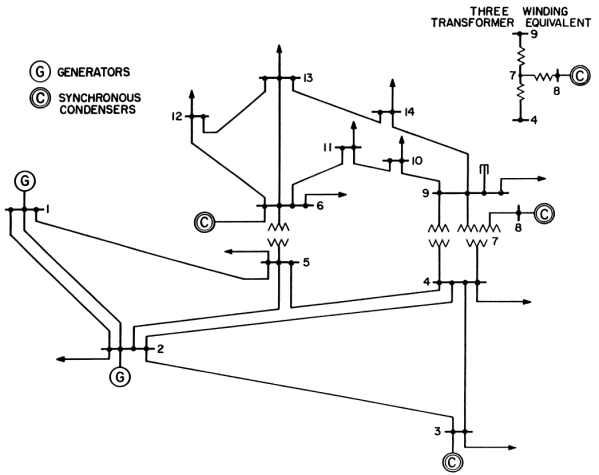
\includegraphics[width=\textwidth]{Single-line-diagram-of-IEEE-14-bus-system.png}
  \caption{IEEE 14 bus system diagram}
\end{figure}

\subsection{Initial Conditions}

The reference angle for the load flow is set at bus n°1. \\

Here are the initial conditions for each generator.

\begin{center}
\begin{tabular}{|c|c|c|c|c|}
  \hline
  Generator & P (MW) & Q (Mvar) & U (kV) & $\Theta$ (°) \\
  \hline
  1 & 232.39 & -16.55 & 73.14 & 0.00\\
  2 & 40.00 & 43.56 & 72.11 & -4.98\\
  3 & 0.00 & 25.07 & 69.69 & -12.73\\
  6 & 0.00 & 12.73 & 14.77 & -14.22\\
  8 & 0.00 & 17.62 & 15.04 & -13.36\\
  \hline
\end{tabular}
\end{center}

\subsection{Models}

\subsubsection{Synchronous Machines}

The following table recaps the modelisation of each generator.

\begin{center}
\begin{tabular}{|c|c|c|c|c|c|}
  \hline
  Generator & Windings  & Saturations & Transformer\\
  \hline
  1 & 4 & Yes & Yes\\
  2 & 4 & Yes & Yes\\
  3 & 4 & Yes & Yes\\
  6 & 3 & Yes & No\\
  8 & 3 & Yes & Yes\\
  \hline
\end{tabular}
\end{center}

All 5 machines are controlled by a proportional speed governor and a proportional voltage regulator. \\

For every machine the voltage regulator is as follows:
\begin{figure}[H]
\centering
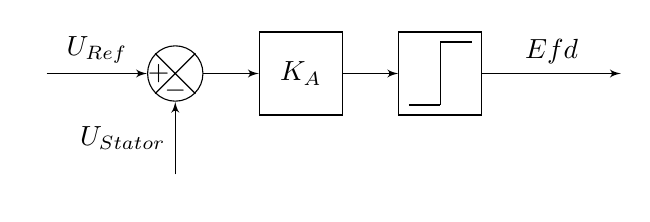
\begin{tikzpicture}
\sbEntree{E}
\sbCompSum[5]{errAVR}{E}{}{-}{+}{}
\sbRelier[$U_{Ref}$]{E}{errAVR}
\sbDecaleNoeudy[4]{errAVR}{Us}
\sbRelier[$U_{Stator}$]{Us}{errAVR}
\sbBloc{Gain}{$K_A$}{errAVR}
\sbRelier{errAVR}{Gain}
\sbBlocL{Limiter}{\tikz {\draw (-0.4,-0.4) -- (0,-0.4);\draw (0,-0.4) -- (0,0.4); \draw (0,0.4) -- (0.4,0.4); }}{Gain}
\sbSortie[5]{S}{Limiter}
\sbRelier[$Efd$]{Limiter}{S}
\end{tikzpicture}
\caption{Voltage regulator}
\end{figure}

For every machine the speed governor is as follows:
\begin{figure}[H]
\centering
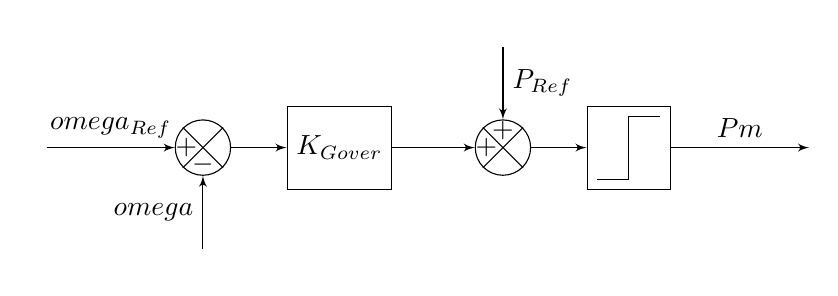
\begin{tikzpicture}
\sbEntree{E}
\sbCompSum[6]{errW}{E}{}{-}{+}{}
\sbRelier[$omega_{Ref}$]{E}{errW}
\sbDecaleNoeudy[4]{errW}{Omega}
\sbRelier[$omega$]{Omega}{errW}
\sbBloc{Gain}{$K_{Gover}$}{errW}
\sbRelier{errW}{Gain}
\sbCompSum{sumP}{Gain}{+}{}{+}{}
\sbRelier{Gain}{sumP}
\sbDecaleNoeudy[-4]{sumP}{PRef}
\sbRelier[$P_{Ref}$]{PRef}{sumP}
\sbBlocL{Limiter}{\tikz {\draw (-0.4,-0.4) -- (0,-0.4);\draw (0,-0.4) -- (0,0.4); \draw (0,0.4) -- (0.4,0.4); }}{sumP}
\sbSortie[5]{S}{Limiter}
\sbRelier[$Pm$]{Limiter}{S}
\end{tikzpicture}
\caption{Speed Governor}
\end{figure}

For every machine the voltage regulator parameters are:
\begin{center}
\begin{tabular}{|c|c|c|c|c|c|}
  \hline
  Generator & $K_{A}$  & $Efd_{Min}$ & $Efd_{Max}$\\
  \hline
  1 & 20 & -5 & 1.44\\
  2 & 20 & -5 & 5\\
  3 & 20 & -5 & 1.115\\
  6 & 20 & -5 & 5\\
  8 & 20 & -5 & 5\\
  \hline
\end{tabular}
\end{center}

For every machine the speed governor parameters are:
\begin{center}
\begin{tabular}{l|l}
   $P_{Nom}=S_{Nom_{SM}}$ & $P_{Max}=S_{Nom_{SM}}$  \\
   $K_{Gover}=5$ & $P_{Min}=0$   \\
\end{tabular}
\end{center}

\subsubsection{System reference frequency}

The system reference frequency used in every machine's model is computed as following:

\[
 \omega_{ref} = \frac{\sum_{Gen \hspace{2pt} n} H_{n} \ Snom_{n} \ \omega_{n}}{\sum_{Gen \hspace{2pt} n} H_{n} \ Snom_{n}}
\]

where $H_{n}$ is generator n inertia and $Snom_{n}$ its apparent power.
\subsubsection{Loads}

Loads follow an alpha beta dynamic behaviour, that is to say :

\[
\begin{aligned}
& P = P_{ref} (\frac{U}{U_{0}})^\alpha \\
& Q = Q_{ref} (\frac{U}{U_{0}})^\beta
\end{aligned}
\]
with $\alpha$ = 1 and $\beta$ = 2 \\

They are either connected through one or two transformers to the grid. Each of these transformers is equipped with a time-changer that can adjust its tap to try to impose a certain voltage.  \\

Loads connected to the 69 kV level are connected behind two transformers with the main following characteristics:
\begin{center}
\begin{tabular}{c|c}
   \textbf{Transmission transformer} & \textbf{Distribution transformer}  \\
   \hline
   \\
   $U_{Target}=1.025 \ pu $ & $U_{Target}=1.015 \ pu $   \\
   $U_{Deadband}=0.01 \ pu $ & $U_{Deadband}=0.01 \ pu $   \\
   $r_{Min}=0.85 $ & $r_{Min}=0.415 $ \\
   $r_{Max}=1.133 $ & $r_{Max}=1.5 $ \\
   $tap_{Min}=0 $ & $tap_{Min}=0 $ \\
   $tap_{Max}=24 $ & $tap_{Max}=84 $ \\
   $t_{1st}=30 \ s $ & $t_{1st}=60 \ s $   \\
   $t_{Next}=10 \ s $ & $t_{Next}=10 \ s $   \\
\end{tabular}
\end{center}

Loads connected to the 13.8 kV level are connected behind one transformer with the main following characteristics:

\begin{center}
\begin{tabular}{c}
   $U_{Target}=1.014 \ pu $  \\
   $U_{Deadband}=0.01 \ pu $ \\
   $r_{Min}=0.9 $ \\
   $r_{Max}=1.1 $ \\
   $tap_{Min}=0 $  \\
   $tap_{Max}=16 $ \\
   $t_{1st}=60 \ s $ \\
   $t_{Next}=10 \ s $  \\
\end{tabular}
\end{center}

\subsection{Solver}
The solver used is a fixed Backward-Euler order 1 solver:
\begin{itemize}
\item $Time step$=1 s
\item $Tolerance$=$10^{-4}$
\end{itemize}

\newpage
\section{Generator disconnections}

\subsection{Additional model and scenario}

In this test case, the generator 3 is equipped with an under voltage automaton with the following parameters: $U_{Monitored} = 1 \ pu $ and $t_{LagAction} = 5 \ s$. It means that if the voltage at the bus 3 stays lower than $1 \ pu$ during $5 \ s$, the generator will be automatically disconnected.\\

The simulated scenario is a disconnection of generator 2 at $ t = 50 s$.

\subsection{Results}

The analysis and the results will focus on two phenomena: first the system evolution in the first seconds following the contingency and then the long-term behavior of the system. \\

For the first phase, the system evolution is mainly driven by the generators behavior. After the disconnection of the generator 2, the other generators (having proportional regulations) immediately try to increase their active and reactive power to compensate for the loss. However, the generators 1 and 3 hit the limitation on their $Efd$ value and are blocked at $Efd_{Max}$. In addition to this, the generator 3 voltage becomes lower than the under voltage automaton limit at $t = 60 \ s$ and at $t = 65 \ s$, the generator is disconnected by this protection, leading to a larger voltage decrease.

\begin{figure}[H]
\subfigure[Generator 1 $Efd$ and $Efd_{Max} \ (pu)$]
{%
  \begin{tikzpicture}
    \begin{axis}[height = 2in]
        \addplot[color=blue!50]
        table[x=time,y=GEN____1_SM_generator_efdPu_value]
        {../IEEE14/IEEE14_GeneratorDisconnections/reference/outputs/curves/curves.csv};
        \addplot[dashed, color=red!50]
        table[x=time,y=GEN____1_SM_voltageRegulator_EfdMaxPu]
        {../IEEE14/IEEE14_GeneratorDisconnections/reference/outputs/curves/curves.csv};
    \legend{$Efd_{Pu}$, $Efd_{{Max}_{Pu}}$}
    \end{axis}
  \end{tikzpicture}
}
\subfigure[Generator 3 $Efd$ and $Efd_{Max} \ (pu)$]
{%
  \begin{tikzpicture}
    \begin{axis}[height = 2in]
        \addplot[color=blue!50]
        table[x=time,y=GEN____3_SM_generator_efdPu_value]
        {../IEEE14/IEEE14_GeneratorDisconnections/reference/outputs/curves/curves.csv};
        \addplot[dashed, color=red!50]
        table[x=time,y=GEN____3_SM_voltageRegulator_EfdMaxPu]
        {../IEEE14/IEEE14_GeneratorDisconnections/reference/outputs/curves/curves.csv};
    \legend{$Efd_{Pu}$, $Efd_{{Max}_{Pu}}$}
    \end{axis}
  \end{tikzpicture}
}
\caption{Generators 1 and 3 efd responses to the generator 2 disconnection}
\end{figure}

\begin{figure}[H]
{
  \begin{tikzpicture}
    \begin{axis}[height = 2 in, xmin = 30, xmax = 100]
        \addplot[color=blue!50]
            table[x=time,y=GEN____3_SM_generator_UPu]
        {../IEEE14/IEEE14_GeneratorDisconnections/reference/outputs/curves/curves.csv};
        \addplot[dashed, color=red!50]
        table[x=time,y=UVA_underVoltageAutomaton_UMinPu]
        {../IEEE14/IEEE14_GeneratorDisconnections/reference/outputs/curves/curves.csv};
    \legend{$U_{Pu}$, $U_{{Min}_{Pu}}$}
    \end{axis}
  \end{tikzpicture}
}
\caption{Voltage evolution on bus 3}
\end{figure}

In the same time, following the disconnections and the voltage decrease, the voltage is lower than the acceptable values for a certain number of transformers connecting the loads to the network. At $t = 80 \ s$, the first transmission transformers begin modifying their tap to restore the load voltage value to its target and at $t = 110 \ s$, the first distribution transformers start acting. This action enables to restore the voltage in an acceptable range for the loads but leads to a more important decrease at the transmission level, without leading in this case to unstability.

\begin{figure}[H]
  \subfigure[Voltage behavior for load 2 transmission transformer]
{
  \begin{tikzpicture}
    \begin{axis}[height = 2 in]
        \addplot[color=blue!50]
            table[x=time,y=_LOAD___2_EC_tapChangerT_UMonitored_value]
        {../IEEE14/IEEE14_GeneratorDisconnections/reference/outputs/curves/curves.csv};
        \addplot[dashed, color=red!50]
        table[x=time,y=_LOAD___2_EC_tapChangerT_UTarget]
        {../IEEE14/IEEE14_GeneratorDisconnections/reference/outputs/curves/curves.csv};
    \legend{$U_{Pu}$, $U_{{Target}_{Pu}}$}
    \end{axis}
  \end{tikzpicture}
  }
  \subfigure[Tap behavior for load 2 transmission transformer]
  {
  \begin{tikzpicture}
    \begin{axis}[height = 2 in]
        \addplot[color=blue!50]
            table[x=time,y=_LOAD___2_EC_tapChangerT_tap_value]
        {../IEEE14/IEEE14_GeneratorDisconnections/reference/outputs/curves/curves.csv};
        \addplot[dashed, color=red!50]
        table[x=time,y=_LOAD___2_EC_tapChangerT_tapMax]
        {../IEEE14/IEEE14_GeneratorDisconnections/reference/outputs/curves/curves.csv};
        \addplot[dashed, color=green!50]
        table[x=time,y=_LOAD___2_EC_tapChangerT_tapMin]
        {../IEEE14/IEEE14_GeneratorDisconnections/reference/outputs/curves/curves.csv};
    \legend{$Tap$, $Tap_{Max}$, $Tap_{Min}$}
    \end{axis}
  \end{tikzpicture}
}
\caption{Load 2 transmission transformer behavior}
\end{figure}

\begin{figure}[H]
  \subfigure[Voltage behavior for load 9 transformer]
{
  \begin{tikzpicture}
    \begin{axis}[height = 2 in]
        \addplot[color=blue!50]
            table[x=time,y=_LOAD___9_EC_tapChanger_UMonitored_value]
        {../IEEE14/IEEE14_GeneratorDisconnections/reference/outputs/curves/curves.csv};
        \addplot[dashed, color=red!50]
        table[x=time,y=_LOAD___9_EC_tapChanger_UTarget]
        {../IEEE14/IEEE14_GeneratorDisconnections/reference/outputs/curves/curves.csv};
    \legend{$U_{Pu}$, $U_{{Target}_{Pu}}$}
    \end{axis}
  \end{tikzpicture}
  }
  \subfigure[Tap behavior for load 9 transformer]
  {
  \begin{tikzpicture}
    \begin{axis}[height = 2 in]
        \addplot[color=blue!50]
            table[x=time,y=_LOAD___9_EC_tapChanger_tap_value]
        {../IEEE14/IEEE14_GeneratorDisconnections/reference/outputs/curves/curves.csv};
        \addplot[dashed, color=red!50]
        table[x=time,y=_LOAD___9_EC_tapChanger_tapMax]
        {../IEEE14/IEEE14_GeneratorDisconnections/reference/outputs/curves/curves.csv};
        \addplot[dashed, color=green!50]
        table[x=time,y=_LOAD___9_EC_tapChanger_tapMin]
        {../IEEE14/IEEE14_GeneratorDisconnections/reference/outputs/curves/curves.csv};
    \legend{$Tap$, $Tap_{Max}$, $Tap_{Min}$}
    \end{axis}
  \end{tikzpicture}
}
  \subfigure[Active power variations for load 9 (pu)]
  {
  \begin{tikzpicture}
    \begin{axis}[height = 2 in]
        \addplot[color=blue!50]
            table[x=time,y=_LOAD___9_EC_load_PPu]
        {../IEEE14/IEEE14_GeneratorDisconnections/reference/outputs/curves/curves.csv};
    \end{axis}
  \end{tikzpicture}
}
  \subfigure[Reactive power variations for load 9 (pu)]
  {
  \begin{tikzpicture}
    \begin{axis}[height = 2 in]
        \addplot[color=blue!50]
            table[x=time,y=_LOAD___9_EC_load_QPu]
        {../IEEE14/IEEE14_GeneratorDisconnections/reference/outputs/curves/curves.csv};
    \end{axis}
  \end{tikzpicture}
}
\caption{Load 9 behavior}
\end{figure}

\begin{figure}[H]
  \subfigure[Voltage on bus 1 (kV)]
  {
  \begin{tikzpicture}
    \begin{axis}[height = 2 in]
        \addplot[color=blue!50]
            table[x=time,y=NETWORK__BUS____1_TN_U_value]
        {../IEEE14/IEEE14_GeneratorDisconnections/reference/outputs/curves/curves.csv};
    \end{axis}
  \end{tikzpicture}
}
  \subfigure[Voltage on bus 5 (kV)]
  {
  \begin{tikzpicture}
    \begin{axis}[height = 2 in]
        \addplot[color=blue!50]
            table[x=time,y=NETWORK__BUS____5_TN_U_value]
        {../IEEE14/IEEE14_GeneratorDisconnections/reference/outputs/curves/curves.csv};
    \end{axis}
  \end{tikzpicture}
}
  \subfigure[Voltage on bus 6 (kV)]
  {
  \begin{tikzpicture}
    \begin{axis}[height = 2 in]
        \addplot[color=blue!50]
            table[x=time,y=NETWORK__BUS____6_TN_U_value]
        {../IEEE14/IEEE14_GeneratorDisconnections/reference/outputs/curves/curves.csv};
    \end{axis}
  \end{tikzpicture}
}
\caption{Voltage evolution on different buses}
\end{figure}

\newpage
\section{Cascading line trippings}

\subsection{Additional models and scenario}

In this test case, three current limit automaton are added to the system on lines Bus2-Bus3, Bus2-Bus4 and Bus2-Bus5. A current limit automaton monitors the current going through a line and if it goes above a certain limit during a predefined time duration, the line is disconnected. These current limit automaton models have the following parameters:

\begin{center}
\begin{tabular}{|c|c|c|}
  \hline
  CurrentLimitAutomaton & $t_{{Lag}_{s}}$  & $I_{{Max}_{Pu}}$\\
  \hline
  CLA\_2\_3 & 60 & 600 \\
  CLA\_2\_4 & 60 & 942 \\
  CLA\_2\_5 & 60 & 724.6 \\
  \hline
\end{tabular}
\end{center}

The simulated scenario is a disconnection of the line between bus 1 and bus 5 at $t = 50 \ s$.

\subsection{Results}

The line Bus1-Bus5 disconnection leads to an increase on the current going through the lines Bus2-Bus3, Bus2-Bus4 and Bus2-Bus5. In particular, the current flowing into Bus2-Bus3 line becomes higher than its maximum value. As a consequence, $60 \ s$ later, the Bus2-Bus3 line is disconnected, which increases even more the current going on the two remaining lines (Bus2-Bus4, Bus2-Bus5). The currents on these lines start to be unacceptable and both lines are finally tripped by their current limit automaton, leading to a split of the system in two networks (Buses 1 and 2 on a separate network, and the other ones on the second network). The second system remains then stable until the end of the simulation.

\begin{figure}[H]
  \subfigure[Current on line 2-3 (A)]
  {
  \begin{tikzpicture}
    \begin{axis}[height = 2 in]
        \addplot[color=blue!50]
            table[x=time,y=NETWORK__BUS____2-BUS____3-1_AC_iSide2]
        {../IEEE14/IEEE14_CascadingLineTrippings/reference/outputs/curves/curves.csv};
        \addplot[dashed, color=red!50]
            table[x=time,y=CLA_2_3_currentLimitAutomaton_IMax]
        {../IEEE14/IEEE14_CascadingLineTrippings/reference/outputs/curves/curves.csv};
        \legend{$I_{kV}$, $I_{{Max}_{kV}}$}
    \end{axis}
  \end{tikzpicture}
}
  \subfigure[Current on line 2-4 (A)]
  {
  \begin{tikzpicture}
    \begin{axis}[height = 2 in]
        \addplot[color=blue!50]
            table[x=time,y=NETWORK__BUS____2-BUS____4-1_AC_iSide2]
        {../IEEE14/IEEE14_CascadingLineTrippings/reference/outputs/curves/curves.csv};
        \addplot[dashed, color=red!50]
            table[x=time,y=CLA_2_4_currentLimitAutomaton_IMax]
        {../IEEE14/IEEE14_CascadingLineTrippings/reference/outputs/curves/curves.csv};
        \legend{$I_{kV}$, $I_{{Max}_{kV}}$}
    \end{axis}
  \end{tikzpicture}
}
  \subfigure[Current on line 2-5 (A)]
  {
  \begin{tikzpicture}
    \begin{axis}[height = 2 in]
        \addplot[color=blue!50]
            table[x=time,y=NETWORK__BUS____2-BUS____5-1_AC_iSide2]
        {../IEEE14/IEEE14_CascadingLineTrippings/reference/outputs/curves/curves.csv};
        \addplot[dashed, color=red!50]
            table[x=time,y=CLA_2_5_currentLimitAutomaton_IMax]
        {../IEEE14/IEEE14_CascadingLineTrippings/reference/outputs/curves/curves.csv};
        \legend{$I_{kV}$, $I_{{Max}_{kV}}$}
    \end{axis}
  \end{tikzpicture}
}
  \subfigure[Current on line 3-4 (A)]
  {
  \begin{tikzpicture}
    \begin{axis}[height = 2 in]
        \addplot[color=blue!50]
            table[x=time,y=NETWORK__BUS____3-BUS____4-1_AC_iSide2]
        {../IEEE14/IEEE14_CascadingLineTrippings/reference/outputs/curves/curves.csv};
    \end{axis}
  \end{tikzpicture}
}
\caption{Current evolution on different lines}
\end{figure}

\chapter{IEEE57}

The IEEE57 bus system is a standard test case in the power system community. It represents a simple approximation of the American Electric Power system (in the U.S. Midwest) as it was in the early 1960s. The data were provided by Iraj Dabbagchi of AEP and converted into the IEEE Common Data Format by Rich Christie at the University of Washington in August 1993.

\textbf{Note. The test case is used in a modified way in this example: arbitrary dynamic data are added.}

\section{Test case description}

The IEEE 57-bus test case system has 57 buses, 7 generators, 3 shunts, 16 transformers, 63 lines and 42 loads.\\
There are three voltage levels in the test case: 69 kV, 18 kV and 13.8 kV. The outer part of the system, with the generators, corresponds to the 69 kV network. The upper inner part is the 18 kV part and the lower inner part is the 13.8 kV part.

\begin{figure}[H]
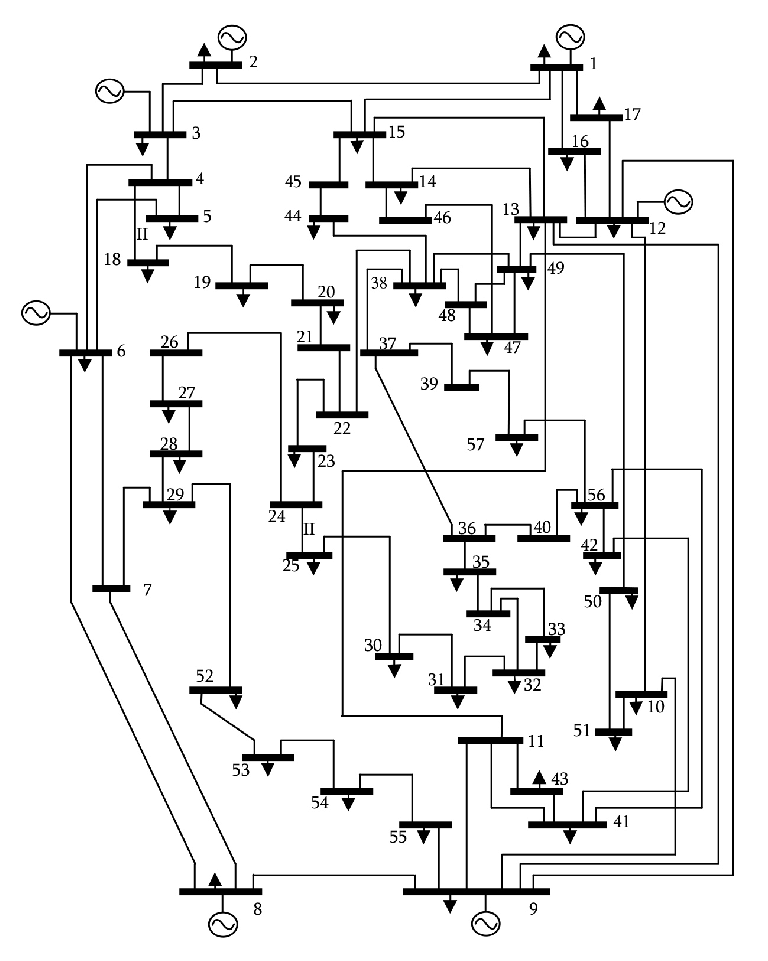
\includegraphics[scale=0.5]{IEEE57BusSystem.png}
\caption{IEEE57 system representation}
\label{circuit-1}
\end{figure}

\subsection{Models}

The generators are modeled as four windings synchronous generators models with a proportional voltage regulator and a proportional speed governor (transformers are included into the machine model; saturations are represented).

The voltage regulator is as follows:
\begin{figure}[H]
\centering
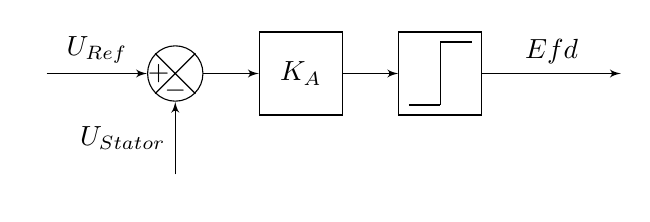
\begin{tikzpicture}
\sbEntree{E}
\sbCompSum[5]{errAVR}{E}{}{-}{+}{}
\sbRelier[$U_{Ref}$]{E}{errAVR}
\sbDecaleNoeudy[4]{errAVR}{Us}
\sbRelier[$U_{Stator}$]{Us}{errAVR}
\sbBloc{Gain}{$K_A$}{errAVR}
\sbRelier{errAVR}{Gain}
\sbBlocL{Limiter}{\tikz {\draw (-0.4,-0.4) -- (0,-0.4);\draw (0,-0.4) -- (0,0.4); \draw (0,0.4) -- (0.4,0.4); }}{Gain}
\sbSortie[5]{S}{Limiter}
\sbRelier[$Efd$]{Limiter}{S}
\end{tikzpicture}
\caption{Voltage regulator}
\end{figure}

The speed governor is as follows - omegaRef being 1 pu in this control scheme -:
\begin{figure}[H]
\centering
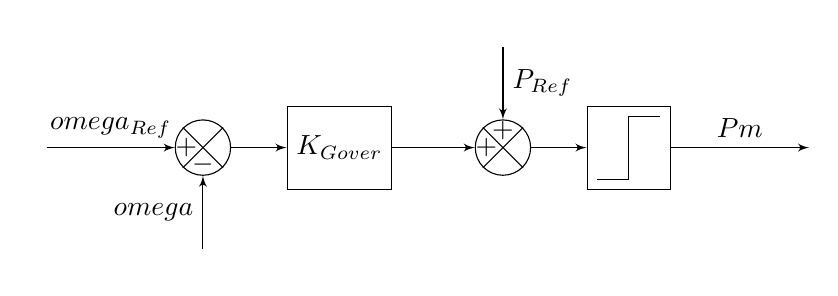
\begin{tikzpicture}
\sbEntree{E}
\sbCompSum[6]{errW}{E}{}{-}{+}{}
\sbRelier[$omega_{Ref}$]{E}{errW}
\sbDecaleNoeudy[4]{errW}{Omega}
\sbRelier[$omega$]{Omega}{errW}
\sbBloc{Gain}{$K_{Gover}$}{errW}
\sbRelier{errW}{Gain}
\sbCompSum{sumP}{Gain}{+}{}{+}{}
\sbRelier{Gain}{sumP}
\sbDecaleNoeudy[-4]{sumP}{PRef}
\sbRelier[$P_{Ref}$]{PRef}{sumP}
\sbBlocL{Limiter}{\tikz {\draw (-0.4,-0.4) -- (0,-0.4);\draw (0,-0.4) -- (0,0.4); \draw (0,0.4) -- (0.4,0.4); }}{sumP}
\sbSortie[5]{S}{Limiter}
\sbRelier[$Pm$]{Limiter}{S}
\end{tikzpicture}
\caption{Speed Governor}
\end{figure}

The loads are modeled as voltage-dependant loads behind one or two transformers equipped with tap-changers:
\begin{equation*}
\begin{aligned}
& P = P_{0} * (\frac{U}{U_{0}})^\alpha \\
& Q = Q_{0} * (\frac{U}{U_{0}})^\beta
\end{aligned}
\label{Voltage-dependant load model}
\end{equation*}

The system reference frequency is calculated by the OmegaRef model using the different generators speeds.\\

All the models parameters can be viewed into the par file available in the test directory.

\subsection{Solver}
The solver used is a fixed Backward-Euler order 1 solver:
\begin{itemize}
\item $Time step$=1 s
\item $Tolerance$=$10^{-4}$
\end{itemize}

\subsection{Scenario}

The simulated scenario is disconnection of the generator 12 at $t = 50 \ s$.

\newpage
\section{Results}

Following the generator disconnection, the voltage decreases on the whole network. In order to restore the load voltage to acceptable values, the transformers begin acting either $30 \ s$ or $60 \ s$ after the contingency.

\begin{figure}[H]
  \subfigure[Voltage behavior for load 1 transmission transformer]
{
  \begin{tikzpicture}
    \begin{axis}[height = 2 in]
        \addplot[color=blue!50]
            table[x=time,y=_LOAD___1_EC_tapChangerT_UMonitored_value]
        {../IEEE57/IEEE57_GeneratorDisconnection/reference/outputs/curves/curves.csv};
        \addplot[dashed, color=red!50]
        table[x=time,y=_LOAD___1_EC_tapChangerT_UTarget]
        {../IEEE57/IEEE57_GeneratorDisconnection/reference/outputs/curves/curves.csv};
    \legend{$U_{Pu}$, $U_{{Target}_{Pu}}$}
    \end{axis}
  \end{tikzpicture}
  }
  \subfigure[Tap behavior for load 1 transmission transformer]
  {
  \begin{tikzpicture}
    \begin{axis}[height = 2 in]
        \addplot[color=blue!50]
            table[x=time,y=_LOAD___1_EC_tapChangerT_tap_value]
        {../IEEE57/IEEE57_GeneratorDisconnection/reference/outputs/curves/curves.csv};
        \addplot[dashed, color=red!50]
        table[x=time,y=_LOAD___1_EC_tapChangerT_tapMax]
        {../IEEE57/IEEE57_GeneratorDisconnection/reference/outputs/curves/curves.csv};
        \addplot[dashed, color=green!50]
        table[x=time,y=_LOAD___1_EC_tapChangerT_tapMin]
        {../IEEE57/IEEE57_GeneratorDisconnection/reference/outputs/curves/curves.csv};
    \legend{$Tap$, $Tap_{Max}$, $Tap_{Min}$}
    \end{axis}
  \end{tikzpicture}
}
\caption{Load 1 transmission transformer behavior}
\end{figure}

\begin{figure}[H]
  \subfigure[Voltage behavior for load 38 transformer]
{
  \begin{tikzpicture}
    \begin{axis}[height = 2 in]
        \addplot[color=blue!50]
            table[x=time,y=_LOAD__38_EC_tapChanger_UMonitored_value]
        {../IEEE57/IEEE57_GeneratorDisconnection/reference/outputs/curves/curves.csv};
        \addplot[dashed, color=red!50]
        table[x=time,y=_LOAD__38_EC_tapChanger_UTarget]
        {../IEEE57/IEEE57_GeneratorDisconnection/reference/outputs/curves/curves.csv};
    \legend{$U_{Pu}$, $U_{{Target}_{Pu}}$}
    \end{axis}
  \end{tikzpicture}
  }
  \subfigure[Tap behavior for load 38 transformer]
  {
  \begin{tikzpicture}
    \begin{axis}[height = 2 in]
        \addplot[color=blue!50]
            table[x=time,y=_LOAD__38_EC_tapChanger_tap_value]
        {../IEEE57/IEEE57_GeneratorDisconnection/reference/outputs/curves/curves.csv};
        \addplot[dashed, color=red!50]
        table[x=time,y=_LOAD__38_EC_tapChanger_tapMax]
        {../IEEE57/IEEE57_GeneratorDisconnection/reference/outputs/curves/curves.csv};
        \addplot[dashed, color=green!50]
        table[x=time,y=_LOAD__38_EC_tapChanger_tapMin]
        {../IEEE57/IEEE57_GeneratorDisconnection/reference/outputs/curves/curves.csv};
    \legend{$Tap$, $Tap_{Max}$, $Tap_{Min}$}
    \end{axis}
  \end{tikzpicture}
}
\caption{Load 38 transformer behavior}
\end{figure}

\begin{figure}[H]
  \subfigure[Voltage on bus 1 (kV)]
  {
  \begin{tikzpicture}
    \begin{axis}[height = 2 in, xmax = 300]
        \addplot[color=blue!50]
            table[x=time,y=NETWORK__KANA___1_TN_U_value]
        {../IEEE57/IEEE57_GeneratorDisconnection/reference/outputs/curves/curves.csv};
    \end{axis}
  \end{tikzpicture}
}
  \subfigure[Voltage on bus 9 (kV)]
  {
  \begin{tikzpicture}
    \begin{axis}[height = 2 in, xmax = 300]
        \addplot[color=blue!50]
            table[x=time,y=NETWORK__SALT___9_TN_U_value]
        {../IEEE57/IEEE57_GeneratorDisconnection/reference/outputs/curves/curves.csv};
    \end{axis}
  \end{tikzpicture}
}
  \subfigure[Voltage on bus 12 (kV)]
  {
  \begin{tikzpicture}
    \begin{axis}[height = 2 in, xmax = 300]
        \addplot[color=blue!50]
            table[x=time,y=NETWORK__GLEN__12_TN_U_value]
        {../IEEE57/IEEE57_GeneratorDisconnection/reference/outputs/curves/curves.csv};
    \end{axis}
  \end{tikzpicture}
}
\caption{Voltage evolution on different buses}
\end{figure}

\end{document}
